\documentclass[../main.tex]{subfiles}

Noch sind die Programme zur Motorsteuerung (Abb. \ref{fig:programm-motorsteuerung}) und Signalerfassung (Abb. \ref{fig:programm-signalerfassung}) getrennt. Weil das Ziel ist, während der Bewegung das Signal aufzunehmen, müssen beide Programme zusammengeführt werden. Das Problem dabei ist, dass die \verb|step| Funktion den Rest des Programms blockiert, solange der Motor läuft. Um dieses Problem zu lösen, wird die Schiene in Intervallen abgefahren, welche von Messungen unterbrochen werden. Wir wählen wieder einen willkürlichen Intervall, beispielsweise \SI{1}{\milli\metre}, und fügen sie den Konstanten des Programms zur Motorsteuerung hinzu.
\begin{figure}[ht]
\begin{lstlisting}[language=C++]
const int interval = 1
\end{lstlisting}
\label{fig:constant-interval}
\end{figure}

\noindent Als nächstes müssen die Motorschritte pro Intervall mit folgender Formel berechnet werden.
\[
    \text{stepsPerInterval} = \frac{\text{interval}}{\text{rangePerRev}} \cdot \text{stepsPerRev}
\]

\noindent\newline Die gesamtanzahl an Intervallen lässt sich folgendermaßen berechnen:

\[
    \text{intervalAmount} = \frac{\text{range}}{\text{interval}}
\]

Mit den obigen Werten \verb|interval|, \verb|stepsPerInterval| und \verb|intervalAmount| können wir nun das gesamte Programm schreiben. Mit einem for-loop soll das Programm durch die Gesamtmenge an Intervallen \verb|intervalAmount| iterieren, und dabei sowohl den Motor um die Anzahl der Schritte pro Intervall \verb|stepsPerInterval| bewegen, als auch das Signal erfassen. Zusätzlich geben wir die Position des Sensors neben der Messung, mit einem Tab seperiert, an.

\begin{figure}[ht]
\begin{lstlisting}[language=C++]
for (int i = 0; i < intervalAmount; i++) {
    stepper.step(stepsPerInterval)
    Serial.println(String(i * measurementInterval) + "  " + String(analogRead(A0)))
}
\end{lstlisting}
\caption{Verbundenes Programm zur Signalerfassung und Motorsteuerung}
\label{fig:programm-signalerfassung-und-motorsteuerung}
\end{figure}

\begin{figure}[ht]
    \centering
    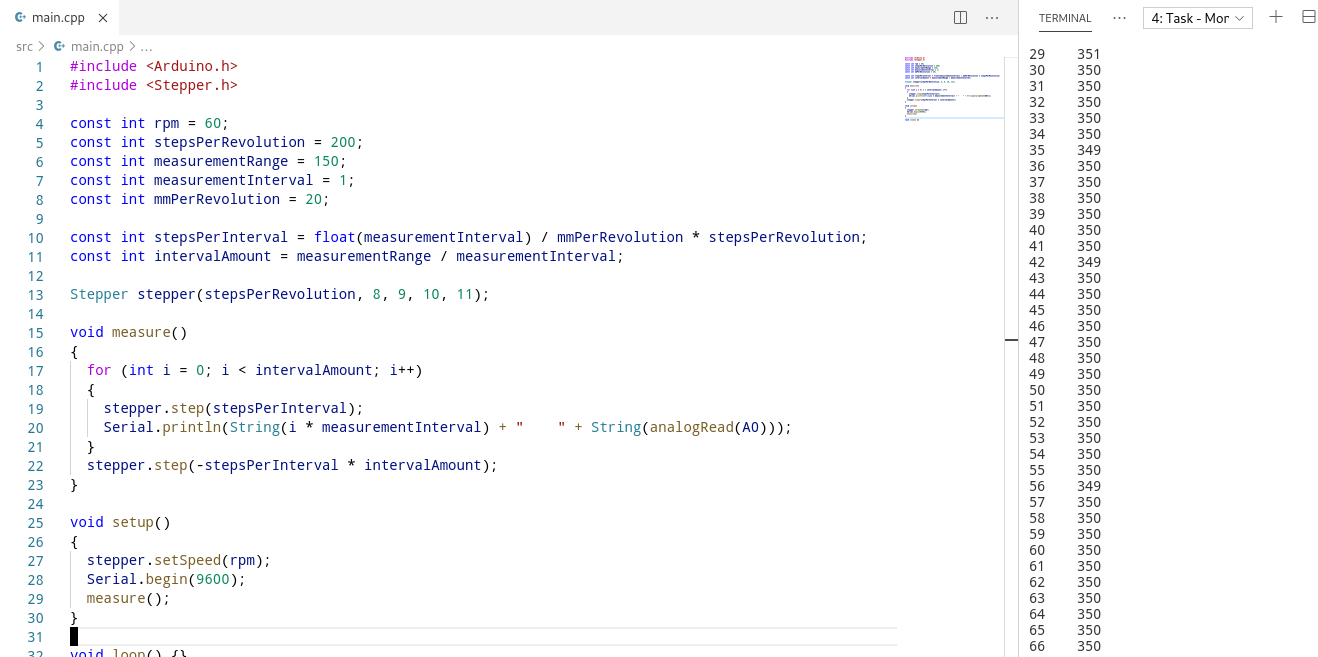
\includegraphics[width=\textwidth]{platformio.png}
    \caption{Gesamtes Programm mit Ausgabe der Daten in der PlatformIO Entwicklungsumgebung (rechts)}
    \label{fig:platformio-signal-simple}
\end{figure}